\chapter{Neutron Configuration}
%Intro\footnotemark\\
\begin{spacing}{1.2}
%note en bas de page
\section{Neutron Setup in Keystone}
\subsection{Adding user or service for Neutron on Keystone}
\par We will start by creating a new Neutron user, assigning him the role of admin,

\\
\begin{figure}[!htb] 
\begin{center} 
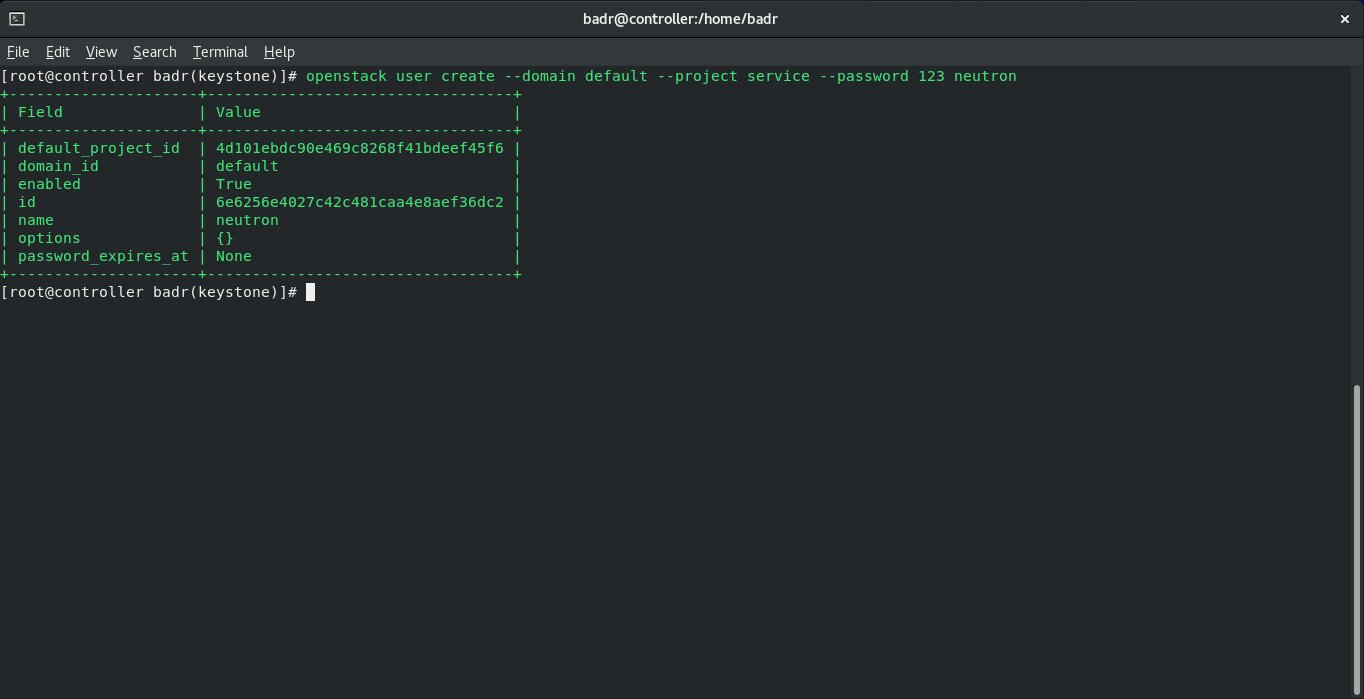
\includegraphics[width=1\linewidth]{Cloud/Neutron Setup in Keystone/create [neutron] user in [service] project} 
\end{center} 
\caption{create [neutron] user in [service] project} 
\end{figure} 
\FloatBarrier
\\
\begin{figure}[!htb] 
\begin{center} 
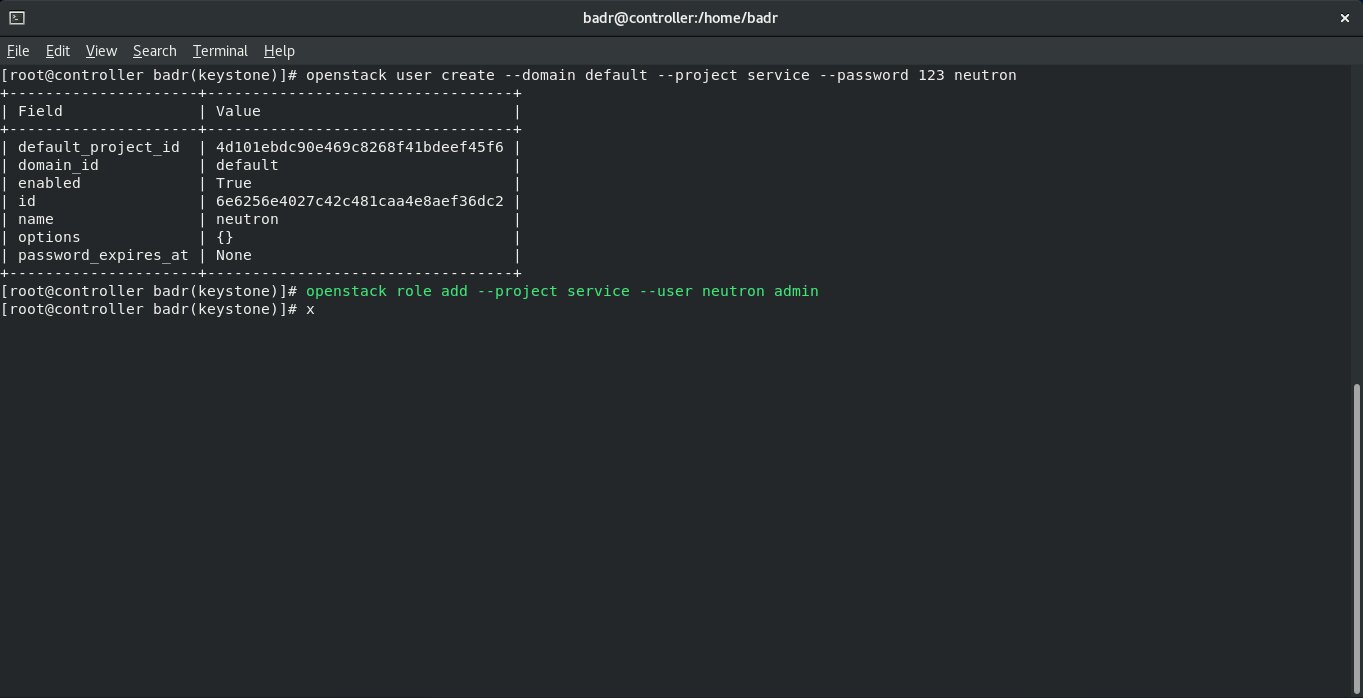
\includegraphics[width=1\linewidth]{Cloud/Neutron Setup in Keystone/add [neutron] user in [admin] role}
\end{center} 
\caption{add [neutron] user in [admin] role} 
\end{figure} 
\FloatBarrier

\par creating a service entry for it, define Neutron API as a host.
\\
\begin{figure}[!htb] 
\begin{center} 
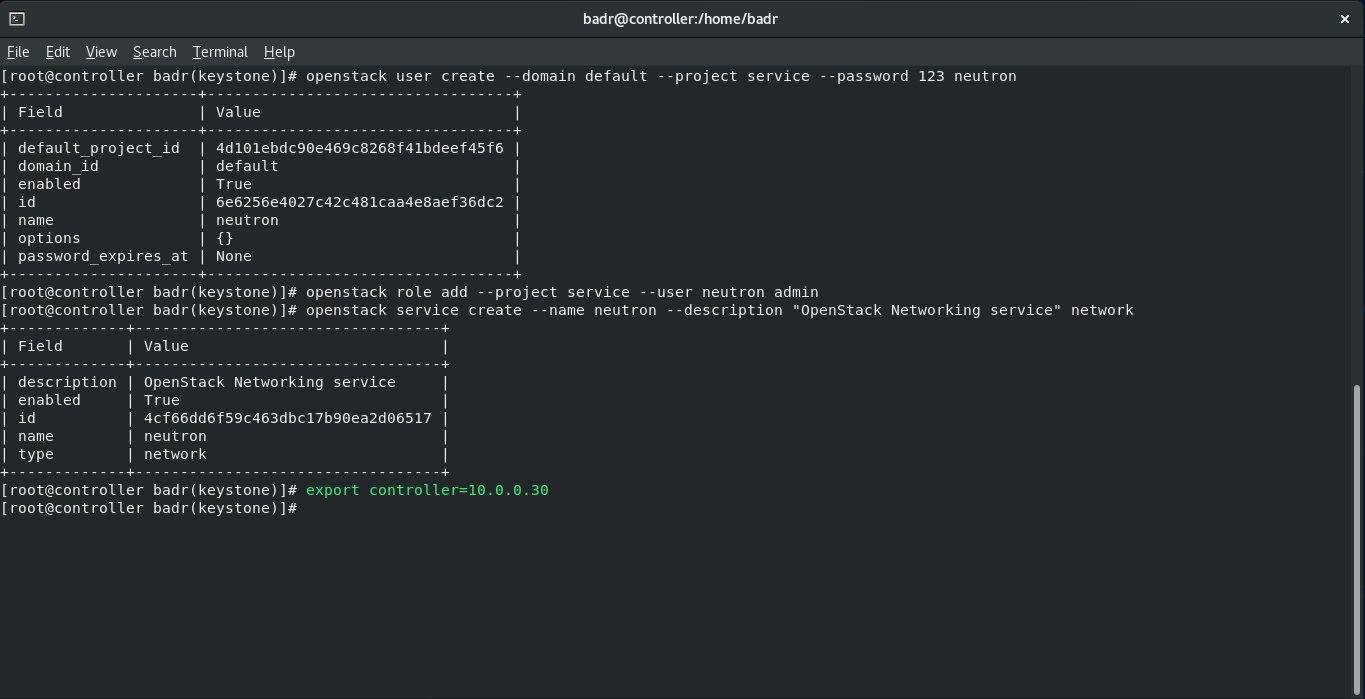
\includegraphics[width=1\linewidth]{Cloud/Neutron Setup in Keystone/define Neutron API Host} 
\end{center} 
\caption{define Neutron API Host} 
\end{figure} 
\FloatBarrier

\par creating an endpoint for the interfaces
public, internal and admin, in order to expose neutron services to our different types of users: 
\\
\begin{figure}[!htb] 
\begin{center} 
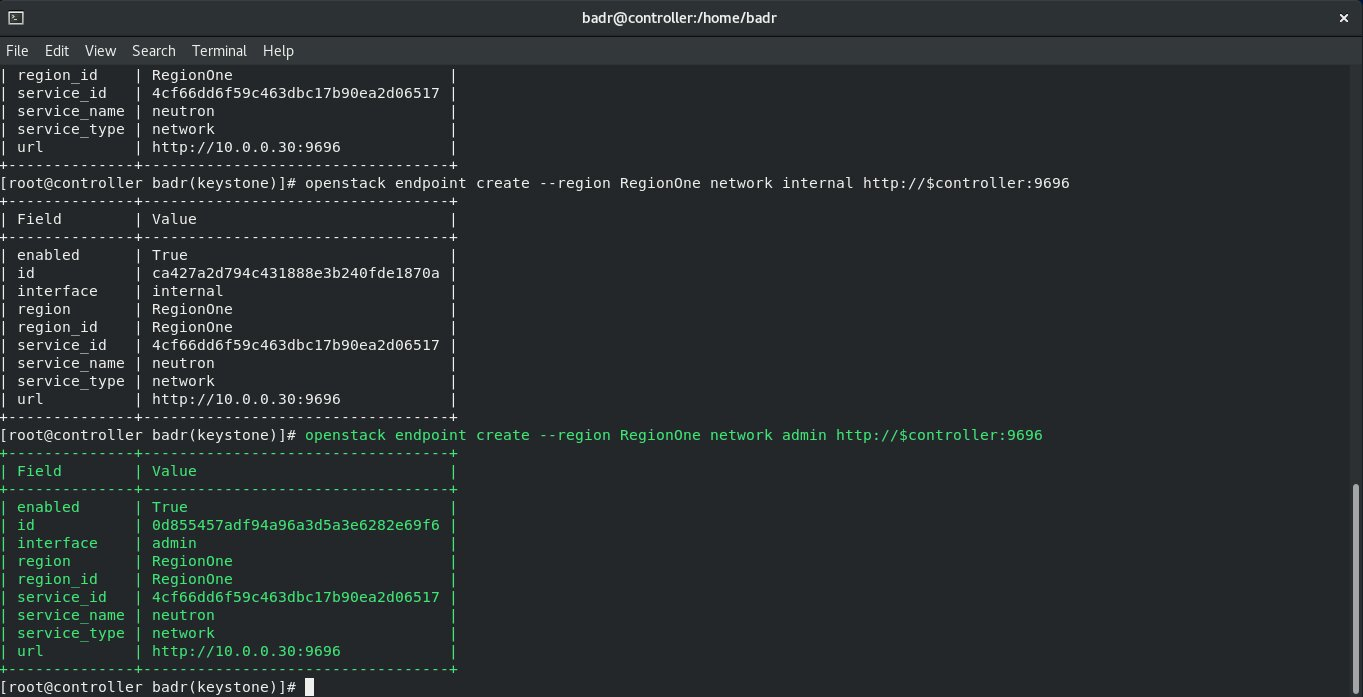
\includegraphics[width=1\linewidth]{Cloud/Neutron Setup in Keystone/create endpoint for [neutron] (admin)} 
\end{center} 
\caption{create endpoint for [neutron] (admin)} 
\end{figure} 
\FloatBarrier

\subsection{Adding a User and Database on MariaDB for Neutron}
\par Next, we'll add this new user to our mariadb database: 
\\
\begin{figure}[!htb] 
\begin{center} 
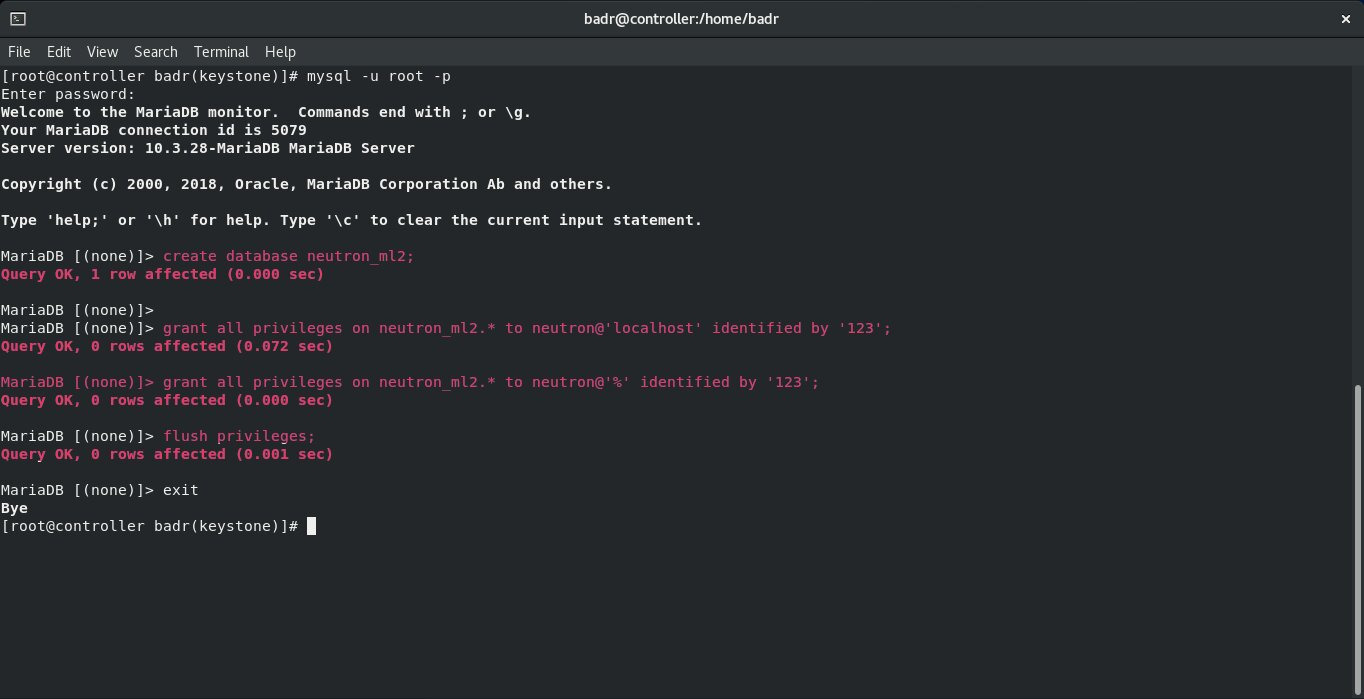
\includegraphics[width=1\linewidth]{Cloud/Neutron Setup in Keystone/Add a User and Database on MariaDB for Neutron} 
\end{center} 
\caption{Add a User and Database on MariaDB for Neutron} 
\end{figure} 
\FloatBarrier


\section{Installing and Configuring Neutron services}
\subsection{Installing Neutron services}

\par Now we will install the services of Neutron to configure them later 
\\
\begin{figure}[!htb] 
\begin{center} 
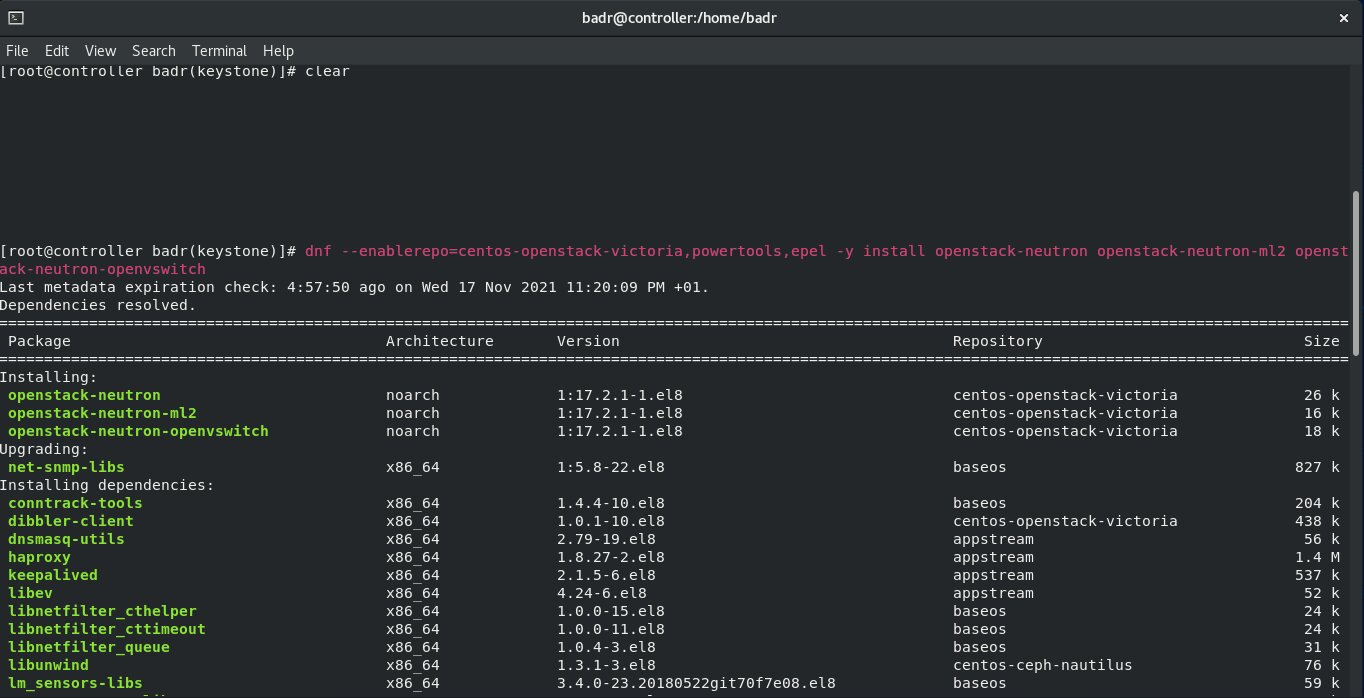
\includegraphics[width=1\linewidth]{Cloud/Installing and Configuring Neutron services/Install Neutron Services 1} 
\end{center} 
\caption{Install Neutron Services 1} 
\end{figure} 
\FloatBarrier
\\

\subsection{Configuring Neutron services}
\par For the configuration, we will rename the file /etc/neutron/neutron.conf.org in \newline
/Etc/neutron/neutron.conf. Here is the contents of the file: 
\\
\begin{figure}[!htb] 
\begin{center} 
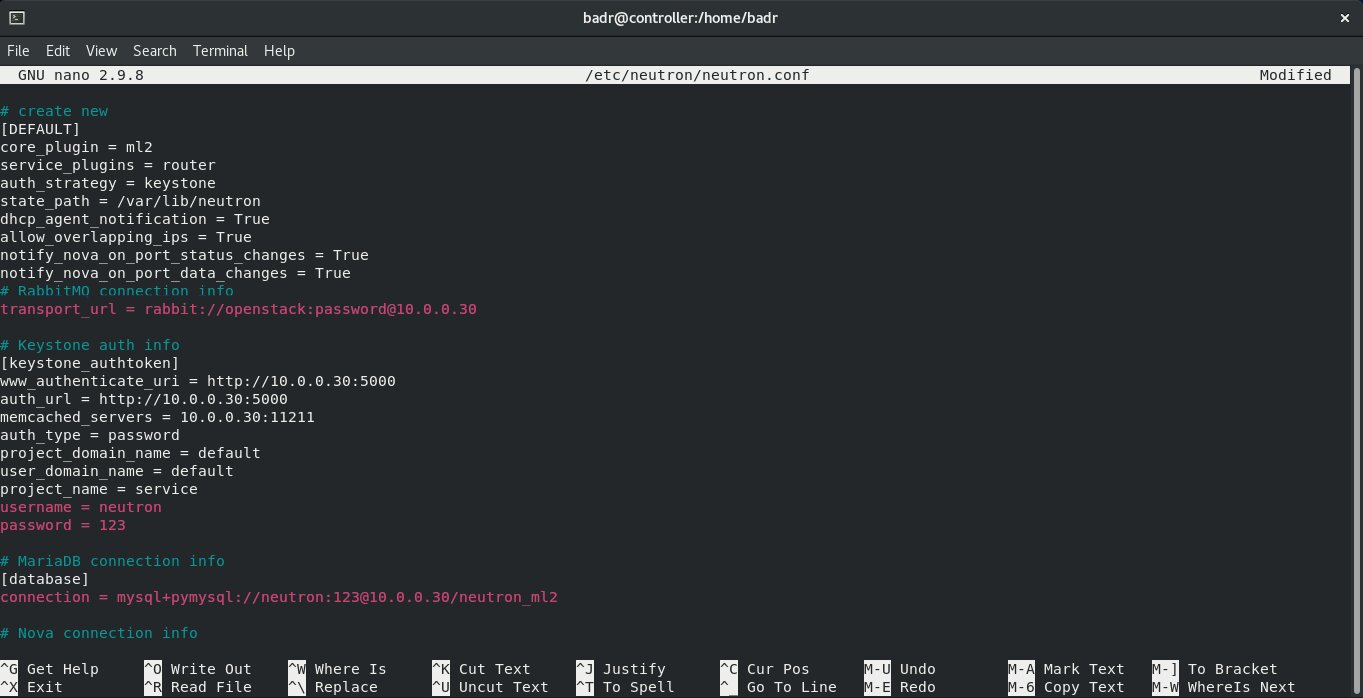
\includegraphics[width=1\linewidth]{Cloud/Installing and Configuring Neutron services/Creating neutron.conf} 
\end{center} 
\caption{Creating neutron.conf} 
\end{figure} 
\FloatBarrier
\\
\par We will change the access permissions to this file with the chmod 640 command. Then we
let's define neutron as a group user.

\par In the / etc / neutron / l3 agent.ini file, we will add the following lines: 
\\
\begin{figure}[!htb] 
\begin{center} 
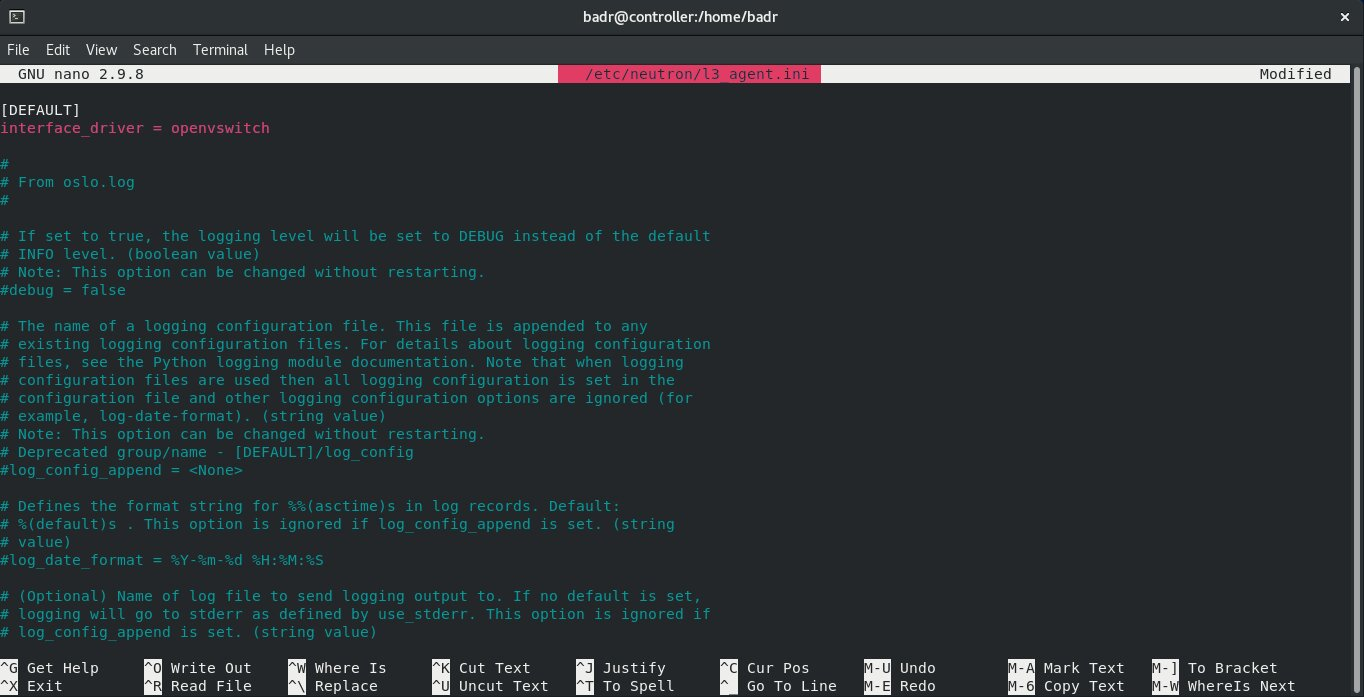
\includegraphics[width=1\linewidth]{Cloud/Installing and Configuring Neutron services/Changing l3_agent.ini} 
\end{center} 
\caption{Changing l3 agent.ini} 
\end{figure} 
\FloatBarrier
\\
\par In the / etc / neutron / dhcp agent.ini file, we will add the following lines: 
\\
\begin{figure}[!htb] 
\begin{center} 
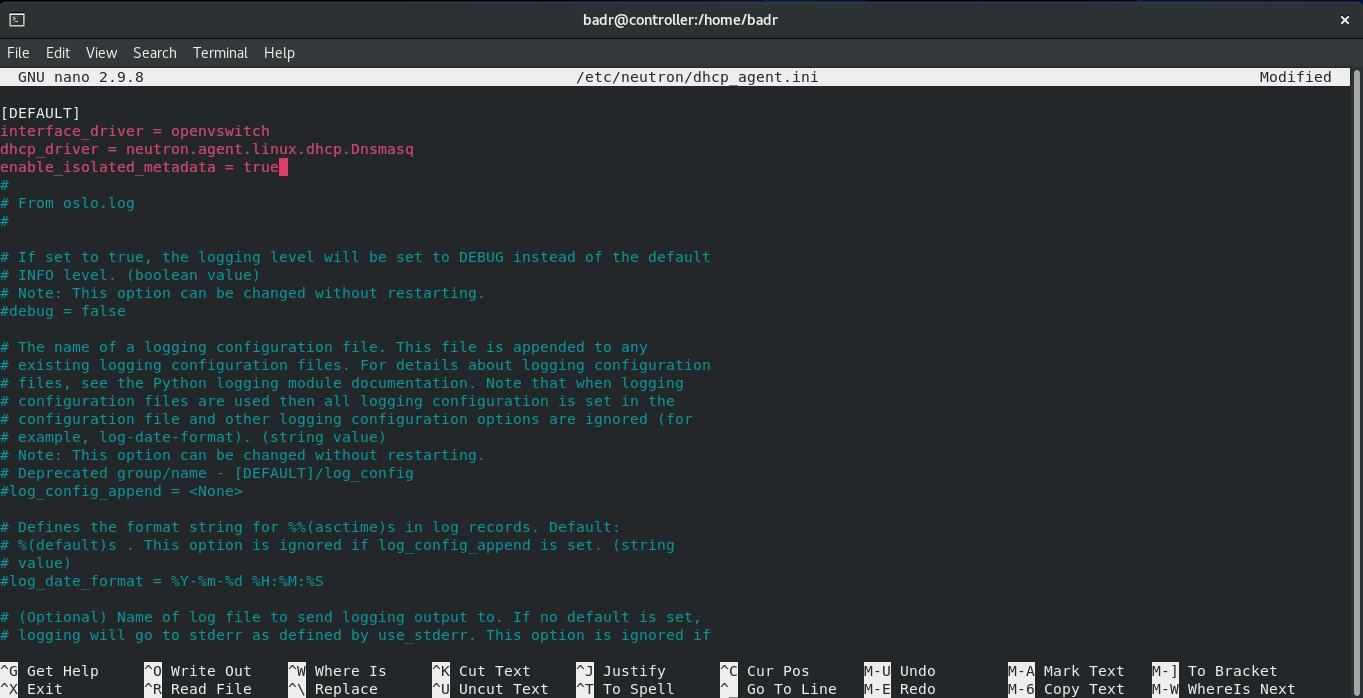
\includegraphics[width=1\linewidth]{Cloud/Installing and Configuring Neutron services/Changing dhcp_agent.ini} 
\end{center} 
\caption{Changing dhcp agent.ini} 
\end{figure} 
\FloatBarrier
\\
\par In the / etc / neutron / metadata agent.ini file, we will add the following code: 
\\
\begin{figure}[!htb] 
\begin{center} 
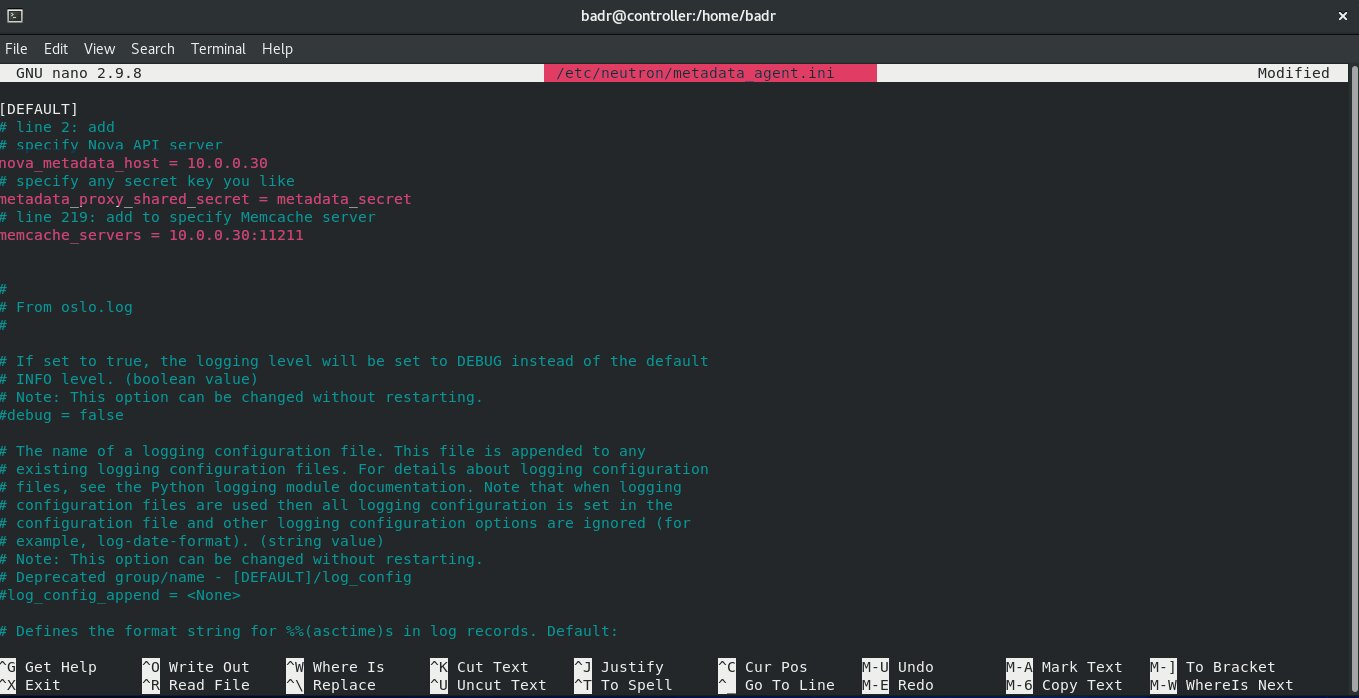
\includegraphics[width=1\linewidth]{Cloud/Installing and Configuring Neutron services/Changing metadata_agent.ini} 
\end{center} 
\caption{Changing metadata agent.ini} 
\end{figure} 
\FloatBarrier
\\
\par In the file / etc / neutron / plugins / ml2 / ml2 conf.ini, we will add the following lines:
\\
\begin{figure}[!htb] 
\begin{center} 
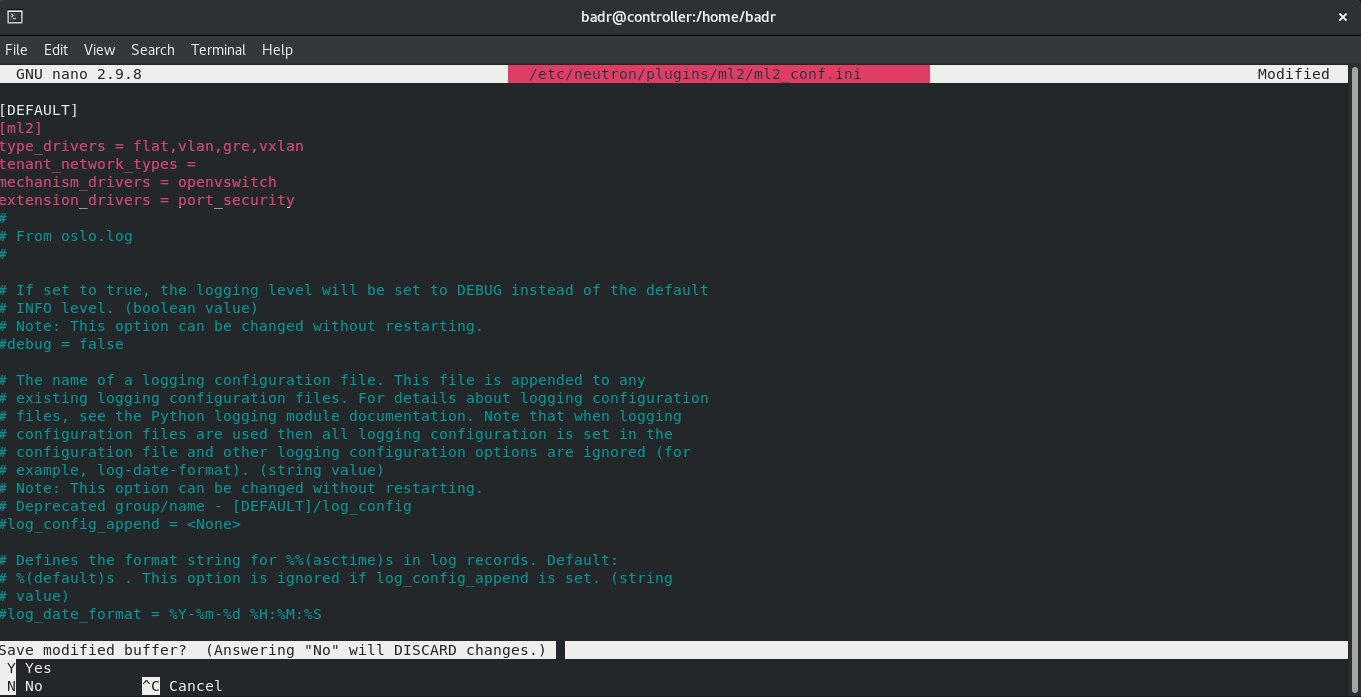
\includegraphics[width=1\linewidth]{Cloud/Installing and Configuring Neutron services/Chaning ml2_conf.ini} 
\end{center} 
\caption{Chaning ml2_conf.ini} 
\end{figure} 
\FloatBarrier
\\
\par In the file / etc / neutron / plugins / ml2 / openvswitch agent.ini, we will add the code
following :
\\
\begin{figure}[!htb] 
\begin{center} 
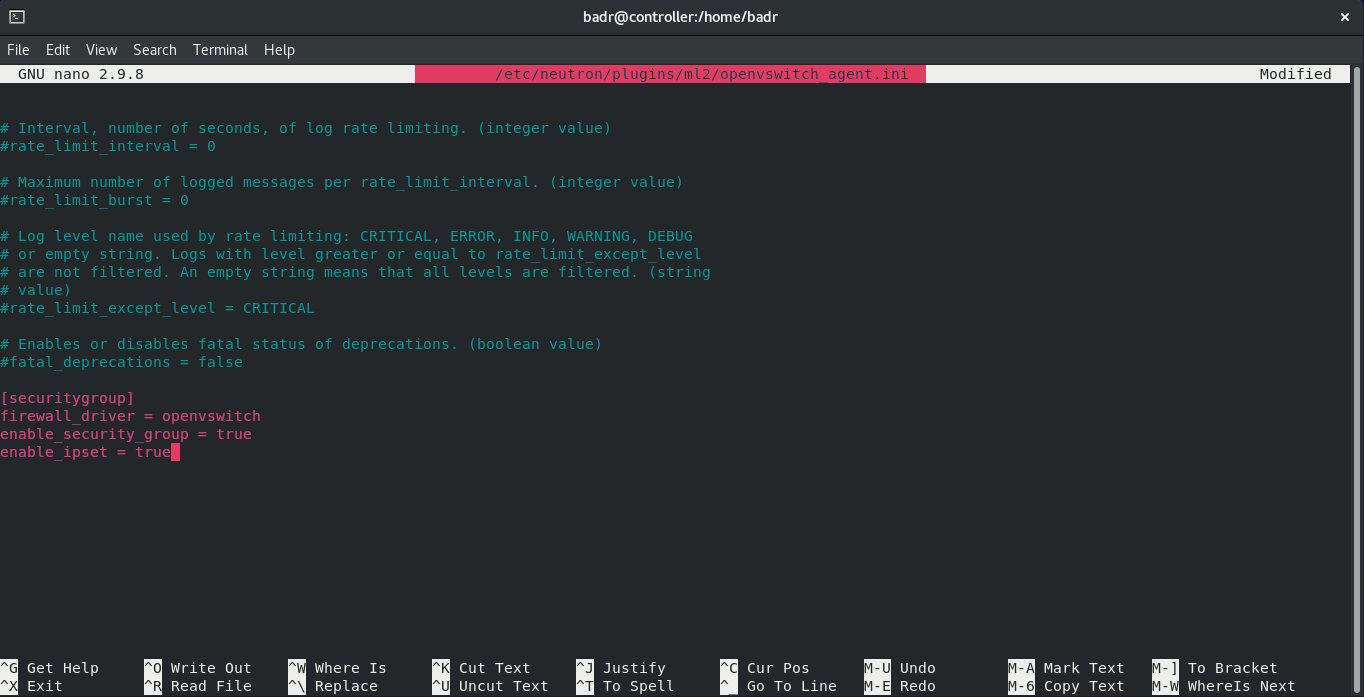
\includegraphics[width=1\linewidth]{Cloud/Installing and Configuring Neutron services/Chaning openvswitch_agent.ini} 
\end{center} 
\caption{Chaning openvswitch agent.ini} 
\end{figure} 
\FloatBarrier
\\
\par Finally in the /etc/nova/nova.conf file, we will add the following lines:
\\
\begin{figure}[!htb] 
\begin{center} 
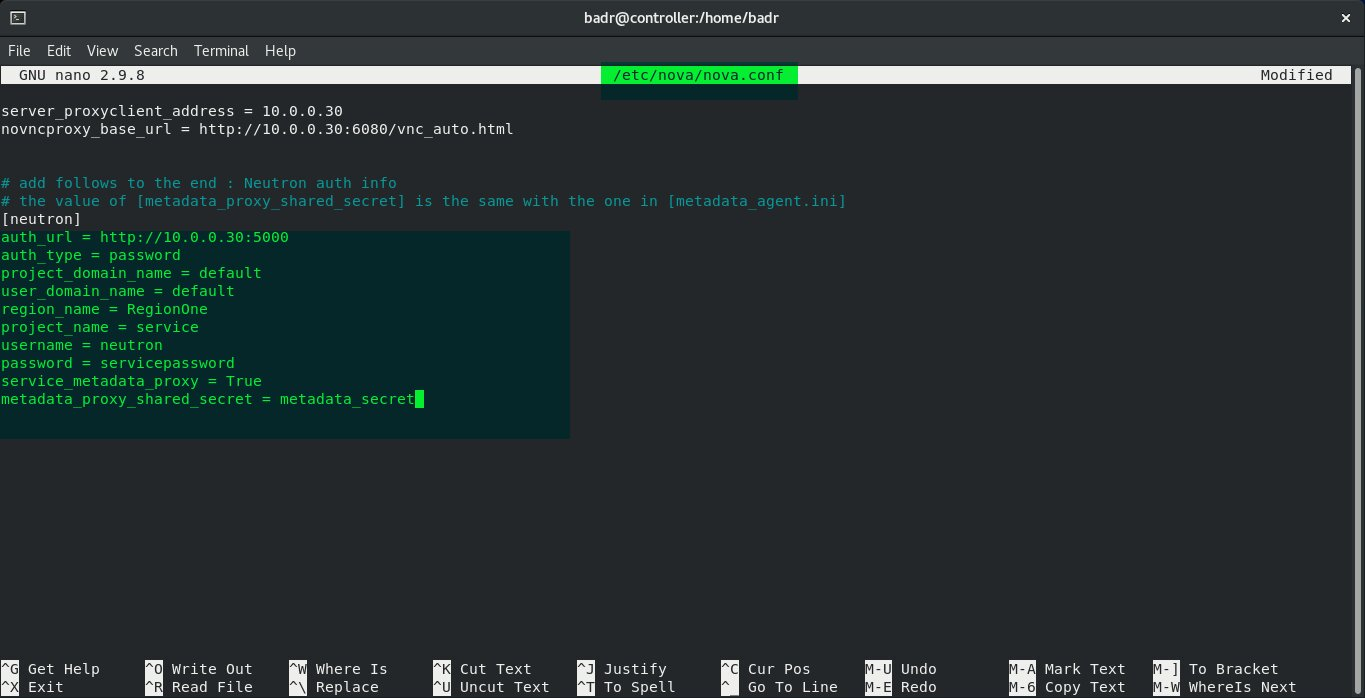
\includegraphics[width=1\linewidth]{Cloud/Installing and Configuring Neutron services/Changing nova.conf} 
\end{center} 
\caption{Changing nova.conf} 
\end{figure} 
\FloatBarrier
\\

\subsection{Starting Neutron services}
\par Enabling the openvswitch service
\\
\begin{figure}[!htb] 
\begin{center} 
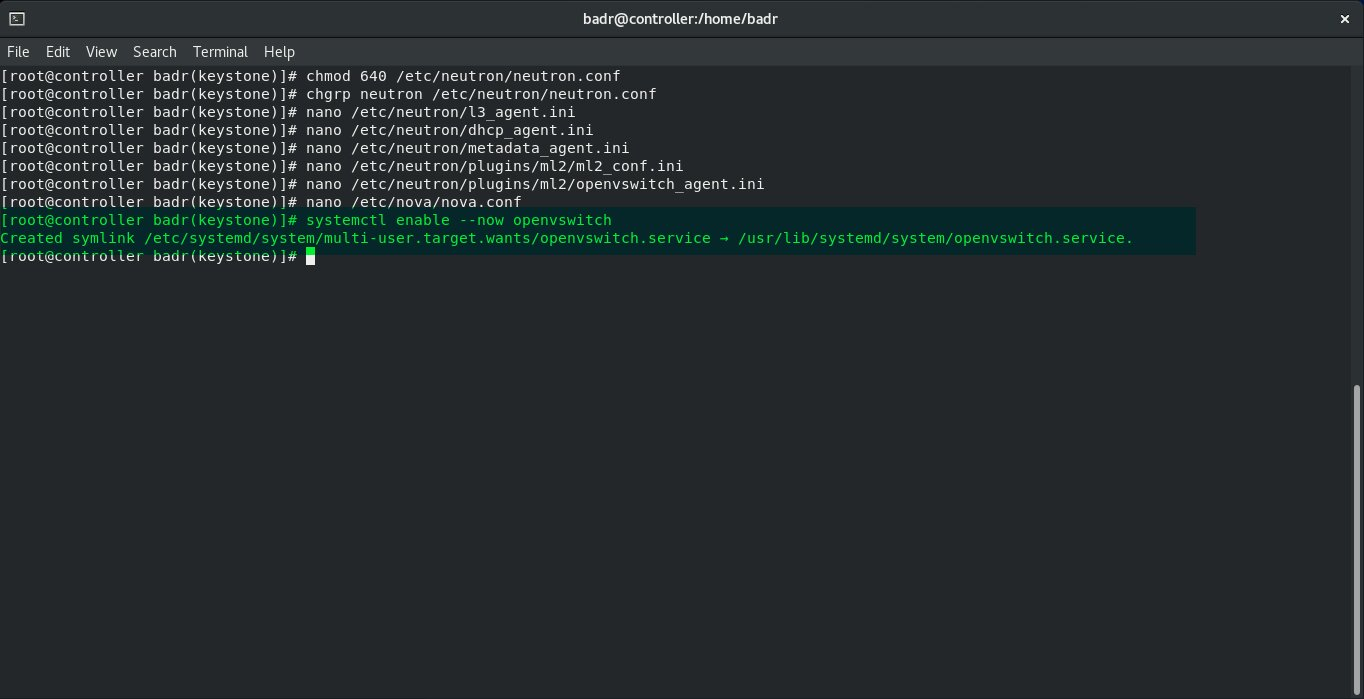
\includegraphics[width=1\linewidth]{Cloud/Installing and Configuring Neutron services/Enabling openvswitch service} 
\end{center} 
\caption{Enabling openvswitch service} 
\end{figure} 
\FloatBarrier
\\

\par Now, we will finally be able to launch the Neutron service: 
\\
\begin{figure}[!htb] 
\begin{center} 
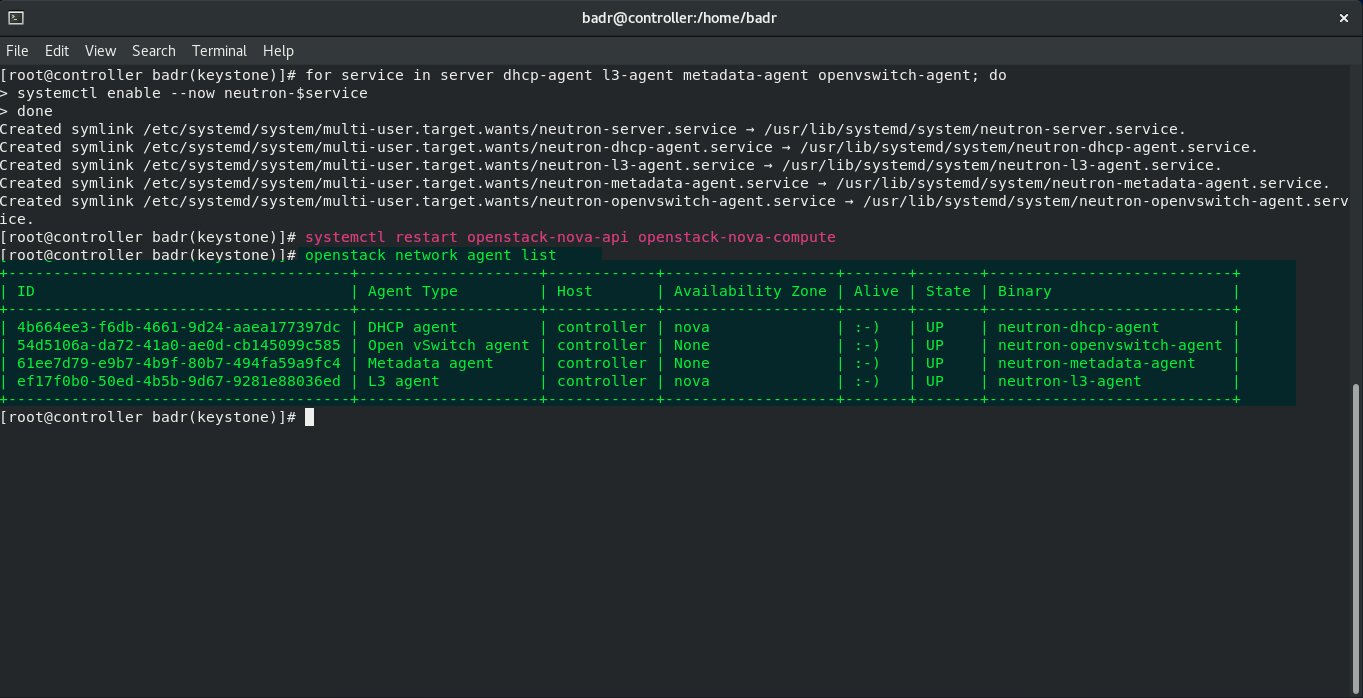
\includegraphics[width=1\linewidth]{Cloud/Installing and Configuring Neutron services/Showing network agents} 
\end{center} 
\caption{Showing network agents} 
\end{figure} 
\FloatBarrier
\\

\section{Configuring Neutron Networking}
\subsection{Configuring Neutron services}
\par It's time to set up the network for Neutron. For this, we will chain these commands, to create a bridge using openvswitch in order to map our vms networks to the actual cloud infrastructure network, the command in green is not working since there is no eth-1 network interface but we should rather use the ens224 network interface, so we simply bridge the eth1 of our vm machines that openstack will create to the network that our ens224 network interface will be connceted to so in order to communicate whit our server instances we should use end-point exposed by the ens224. and openvswitch will map our request to the correspondent eth-1 in our server instances internal virtual network
\\
\begin{figure}[!htb] 
\begin{center} 
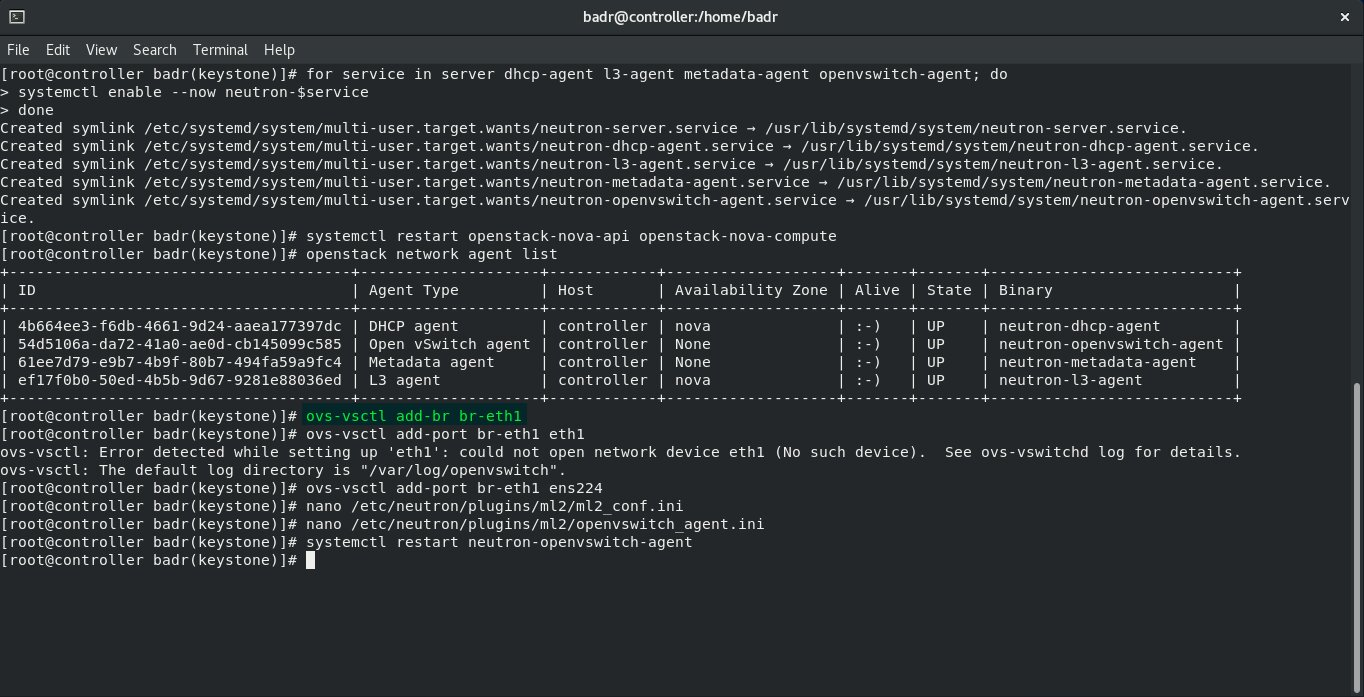
\includegraphics[width=1\linewidth]{Cloud/Configuring Neutron Networking/add bridge} 
\end{center} 
\caption{add bridge} 
\end{figure} 
\FloatBarrier
\\
\par we have to add the following at the end of the ml2_conf.ini and openvswitch_agent.ini files.
\\
\begin{figure}[!htb] 
\begin{center} 
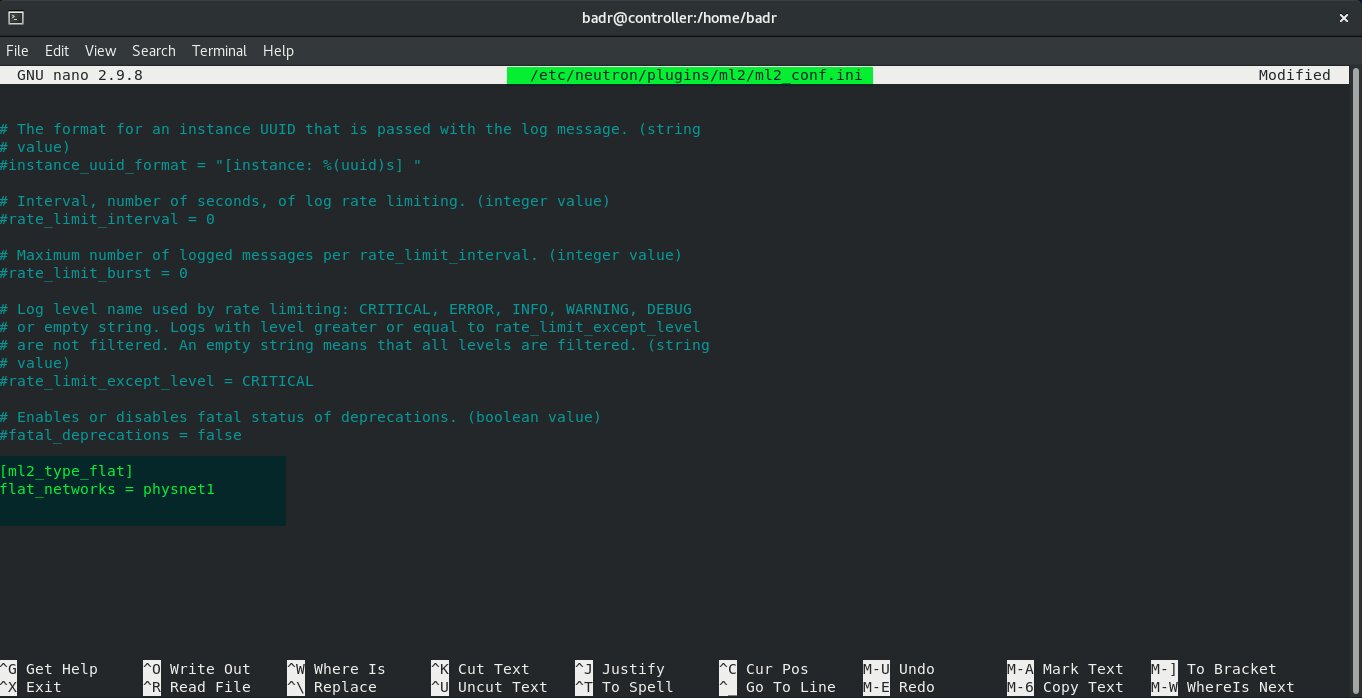
\includegraphics[width=1\linewidth]{Cloud/Configuring Neutron Networking/add to the end of ml2_conf} 
\end{center} 
\caption{add to the end of ml2_conf} 
\end{figure} 
\FloatBarrier
\begin{figure}[!htb] 
\begin{center} 
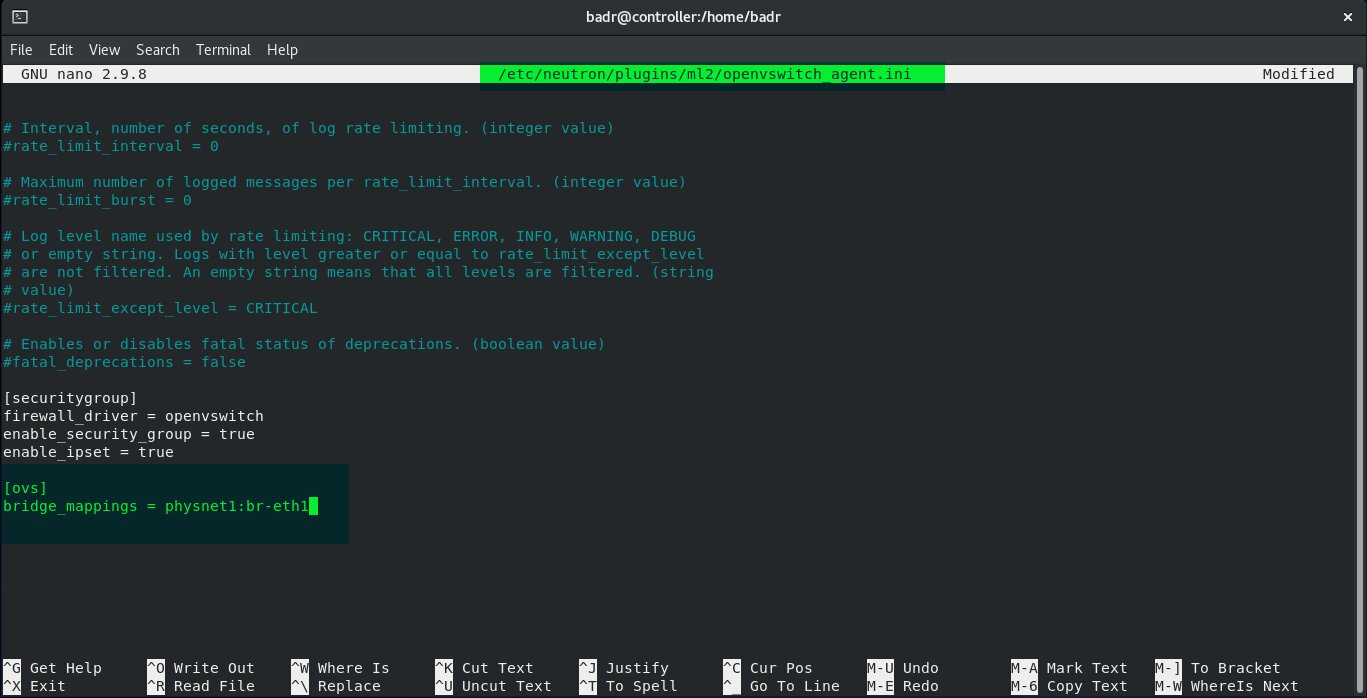
\includegraphics[width=1\linewidth]{Cloud/Configuring Neutron Networking/add to the end of openvswitch-agent} 
\end{center} 
\caption{add to the end of openvswitch-agent} 
\end{figure} 
\FloatBarrier

\subsection{Creating virtual network}
\par We will then create a virtual network named sharednet1: 
\\
\begin{figure}[!htb] 
\begin{center} 
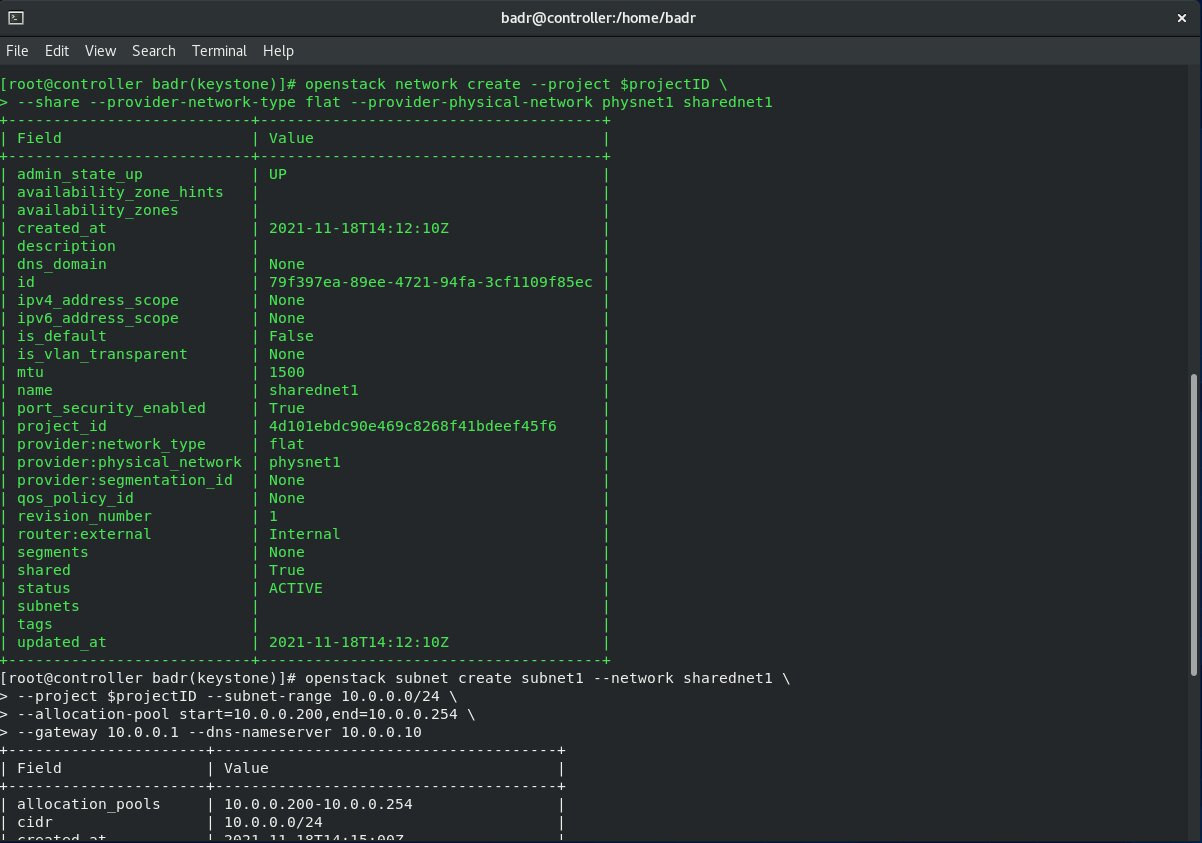
\includegraphics[width=1\linewidth]{Cloud/Configuring Neutron Networking/create network named [sharednet1]} 
\end{center} 
\caption{create network named [sharednet1]} 
\end{figure} 
\FloatBarrier

\par We are going to create a 10.0.0.0/24 subnet for the sharednet1 network: 
\\
\begin{figure}[!htb] 
\begin{center} 
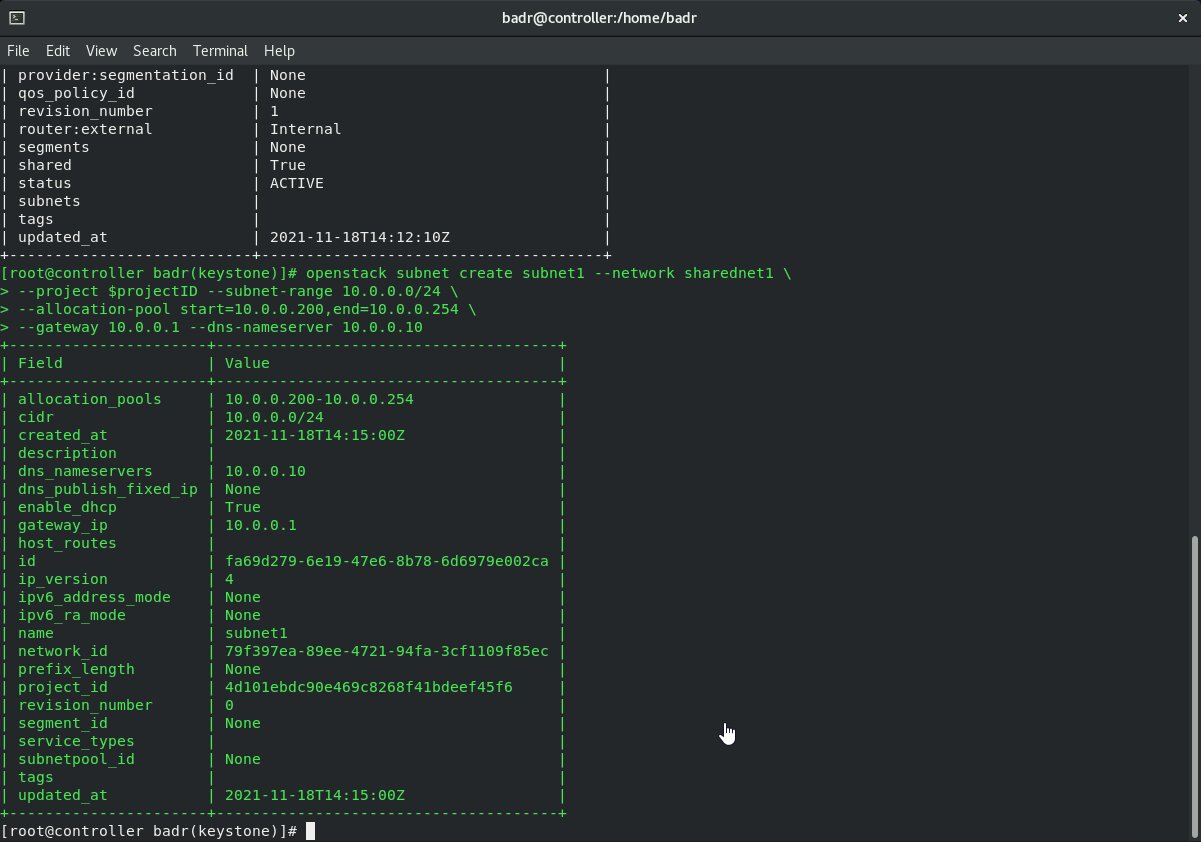
\includegraphics[width=1\linewidth]{Cloud/Configuring Neutron Networking/create subnet [10.0.0.024] in [sharednet1]} 
\end{center} 
\caption{create subnet [10.0.0.024] in [sharednet1]} 
\end{figure} 
\FloatBarrier

\par Finally, we will confirm these parameters:
\\
\begin{figure}[!htb] 
\begin{center} 
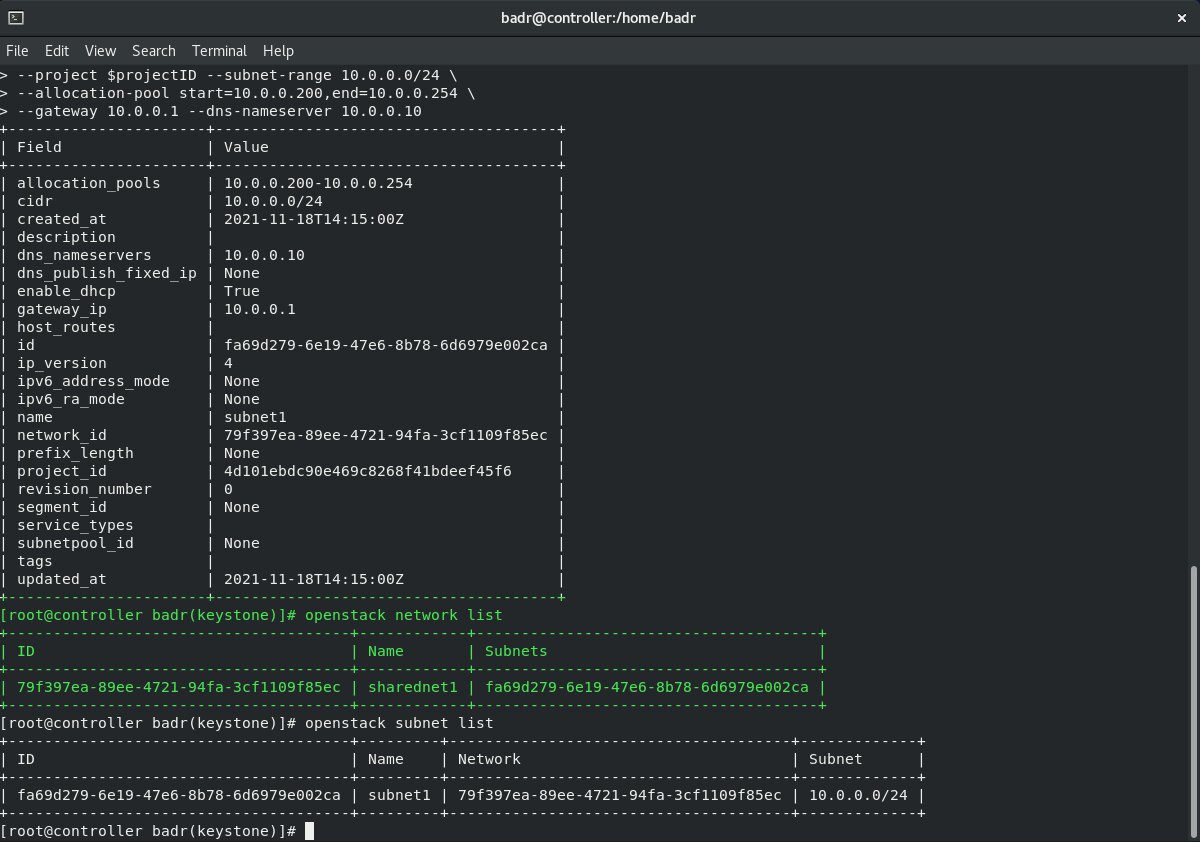
\includegraphics[width=1\linewidth]{Cloud/Configuring Neutron Networking/confirm network list} 
\end{center} 
\caption{confirm network list} 
\end{figure} 
\FloatBarrier


\end{spacing}